%%%%%%%%%%%%%%%%%%%%%%%%%%%%%%%%%%%%%%%%
%%%%%  Chapitre Graphiques
%%%%%%%%%%%%%%%%%%%%%%%%%%%%%%%%%%%%%%%%

\chapter{Les graphiques}

Comme vu en page~\pageref{images}, le paquet \paquet{graphicx} permet d'insérer des images. Mais \LaTeX\ peut faire mieux : il est possible de le faire dessiner. Pour cela, deux grands paquets existent : \paquet{pstricks} et \paquet{tikz}. Le premier, plus ancien, dispose de plus de fonctionnalités diverses développées par différents amateurs au fil des années, tandis que le second est censé être plus précis pour ce qui est des définitions. Les deux sont ici présentés sur des cas similaires pour illustrer leur syntaxe respective. 

\section{PsTricks} \label{pstricks} \incise{---}{---}{325--348}

Les éléments présentés ci-après se basent sur un paquet étendant largement les capacités graphiques rudimentaires de \LaTeX\ : \paquet{pstricks} de Timothy \textsc{Van Zandt}. Sont illustrées ici des bases de fonctionnement. Les lecteurs intéressés sont invités à se tourner vers la documentation accompagnant \paquet{pstricks}.

Ce paquet met à disposition un environnement pour traiter les figures\footnote{Il est cependant possible de tracer \emph{directement} dans le texte les graphiques... mais avec de nombreuses surprises à la clé en terme d'affichage.} : 

\begin{codesimple}{L'environnement de \pseudopaquet{pstricks}}{environnementpstricks}
\begin{pspicture}(§oc£¤largeur§fc,§oc£¤hauteur§fc) 
% Figure pstricks
\end{pspicture}
\end{codesimple}


Dans \paquet{pstricks}, l'unité de mesure est le centimètre. Cet environnement définit ici une zone de \og \emph{largeur} cm $\times$ \emph{hauteur} cm \fg dans laquelle se feront nos tracés.


\subsection{Le placement}

Avant de présenter les objets propres à \paquet{pstricks}, nous manipulons ici un objet bien connu : du texte. Comme tout objet graphique, il peut être positionné dans une figure avec la commande \macro{rput[{\it position}]\{{\it angle}\}({\it x},{\it y})\{{\it objet}\}}. La coordonnée \macron{({\it x},{\it y})}, présentée par une croix bleue dans l'exemple qui suit, sert de référence au placement de l'objet en suivant la consigne de \emph{position} donnée (l'absence de position centrant l'objet sur cette coordonnée). L'exemple illustre le sens des positions \macron{b}(bottom), \macron{t}(top), \macron{r}(right) et \macron{l}(left). Enfin, l'\emph{angle}, exprimé en degrés (sens trigonométrique), exprime l'angle de la rotation appliquée à l'objet.

\begin{codedoublefig}{Placements et redimensionnements}{dessincouleur}
\begin{pspicture}(10,2)
\psdots[dotstyle=BoldMul,linecolor=bleu6](1,0.5)(0.8,1.1)(8,1.1)(6,1)
\rput(1,0.5){1.\LaTeX}
\rput[bl](0.8,1.1){\resizebox{3.5cm}{!}{2.\textcolor{bleu5}{\LaTeX}}}
\rput{160}(8,1.1){\resizebox{!}{0.7cm}{3.\LaTeX}}
\rput[tr](6,1){\resizebox{!}{0.6cm}{\reflectbox{4.\LaTeX}}}
\end{pspicture}
\end{codedoublefig}
%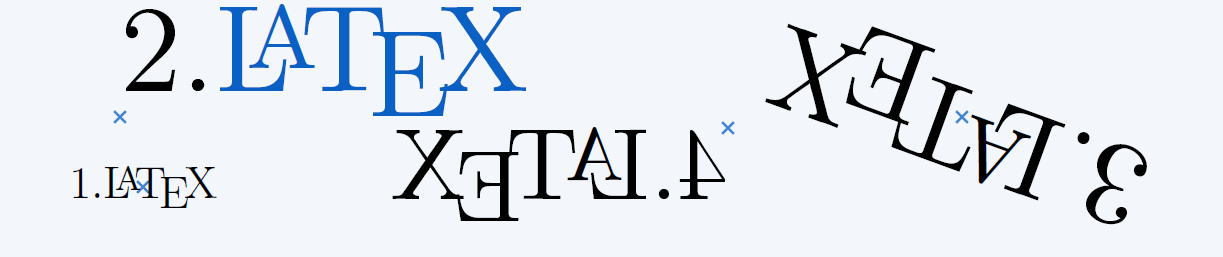
\includegraphics[width=10cm]{images/pstricks1.jpg}

\subsection{Les boîtes} \label{psboites}

Plusieurs commandes permettent d'entourer les objets. L'exemple qui suit illustre les boîtes \macro{psframebox}, \macro{psdiabox} et \macro{pscirclebox}. Les versions étoilées des boîtes permettent de les remplir\footnote{Par défaut, le remplissage est blanc uni. Ainsi, l'étoile est ici strictement équivalente à l'option \macron{fillstyle=solid}.}. L'exemple présente également la manière de saisir des options de présentation avec \paquet{pstricks} : en listant les options entre crochets sous la forme \macron{\it option = valeur} et en séparant les différentes options par des virgules. Ces options permettent, entre autres, de gérer des paramètres comme l'épaisseur de trait, le type de trait, de remplissage ou la couleur.

\begin{codedoublefig}{Boîtes}{pstricksboites}
\begin{pspicture}(10,2)
\rput(2,1){\psframebox{1.\LaTeX}}
\rput(5,0.5){\psframebox*[fillcolor=bleu6,shadow=true]{2.\LaTeX}}
\rput(5,1.5){\psdiabox[linecolor=bleu6]{3.\LaTeX}}
\rput(8,1){\pscirclebox[linestyle=dotted,linecolor=bleu6]{\Large 4.\LaTeX}}
\end{pspicture}
\end{codedoublefig}
%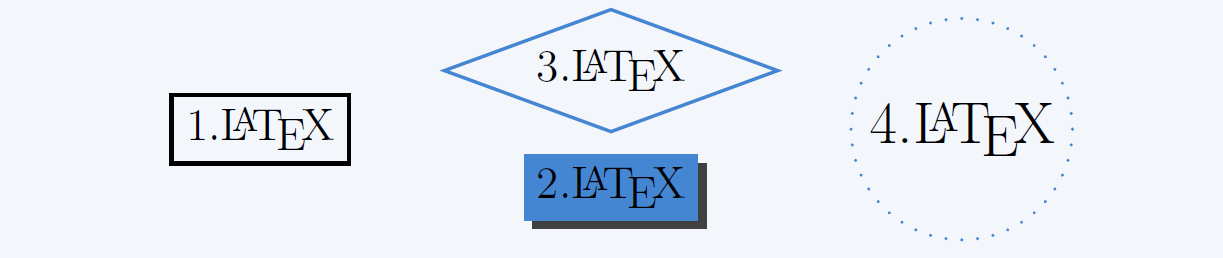
\includegraphics[width=10cm]{images/pstricks2.jpg}

\subsection{Les grilles}

Des grilles peuvent être créées aisément avec différents paramétrages. L'exemple qui suit illustre également une autre manière d'introduire la zone de tracé par l'environnement \macron{pspicture} : la donnée des coordonnées du point inférieur gauche et du point supérieur droit du cadre.

\begin{codedoublefig}{Grilles}{pstricksgrilles}
\begin{pspicture}(-0.5,-0.5)(9.5,1.5)
\psgrid(2,1.4)
\rput(3.5,0){\psgrid[griddots=10,subgriddiv=3,subgridcolor=bleu6](2,1.4)}
\rput(7,0){\psgrid[gridwidth=0.07,subgriddiv=0](2,1.4)}
\end{pspicture}
\end{codedoublefig}
%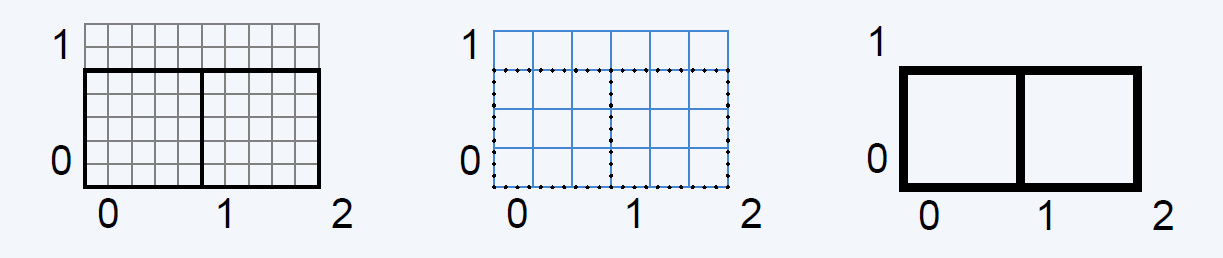
\includegraphics[width=10cm]{images/pstricks3.jpg}

\subsection{Les points et courbes}

De la même manière, \paquet{pstricks} dispose de plusieurs commandes de base pour former des traits anguleux, curvilignes. L'exemple suivant les présente sans option.

\begin{codedoublefig}{Points et courbes}{pstrickspoints}
\begin{pspicture}(-0.25,-0.5)(9.75,1.5)
\psdots(0,1)(0.5,0)(1,0.5)(1.5,0)(2,1)
\psline(2.5,1)(3,0)(3.5,0.5)(4,0)(4.5,1)
\pscurve(5,1)(5.5,0)(6,0.5)(6.5,0)(7,1)
\psccurve(7.5,1)(8,0)(8.5,0.5)(9,0)(9.5,1)
\end{pspicture}
\end{codedoublefig}
%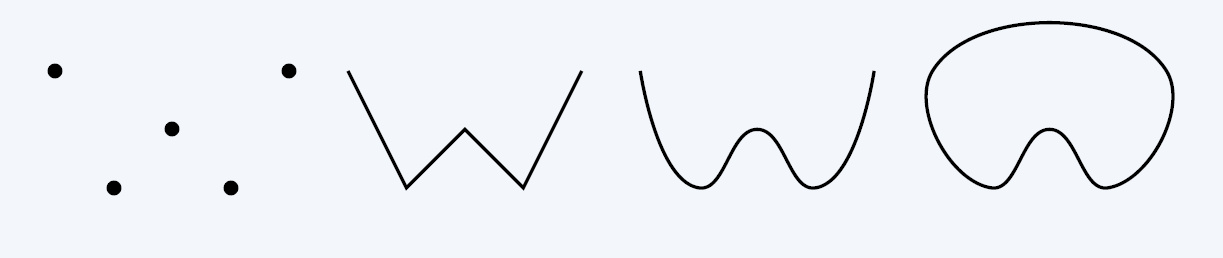
\includegraphics[width=10cm]{images/pstricks4.jpg}


\subsection{Les flèches et options}

Points et courbes peuvent être modifiés en donnant leur épaisseur mais aussi leur forme. Dans le cas du trait, il s'agit de la forme aux extrémités, ce qui permet en particulier d'obtenir les flèches.

\begin{codedoublefig}{Options sur points et courbes}{pstricksoptions}
\begin{pspicture}(-0.25,-0.5)(9.75,1.5)
\psdots[dotstyle=square*](0,1)(2,1)
\psdots[dotstyle=triangle,dotsize=0.2](0.5,0.2)(1,0.7)(1.5,0.2)
\psline[doubleline=true](2.5,0.7)(3,-0.3)(3.5,0.2)(4,-0.3)(4.5,0.7)
\psline[linewidth=0.1](2.5,1.3)(3,0.3)(3.5,0.8)(4,0.3)(4.5,1.3)
\pscurve[linecolor=bleu6]{|-*}(5,0.7)(5.5,-0.3)(6,0.2)(6.5,-0.3)(7,0.7)
\pscurve[arrowscale=2]{->}(5,1.3)(5.5,0.3)(6,0.8)(6.5,0.3)(7,1.3)
\psccurve*[linecolor=bleu6](7.5,1)(8,0)(8.5,0.5)(9,0)(9.5,1)
\end{pspicture}
\end{codedoublefig}
%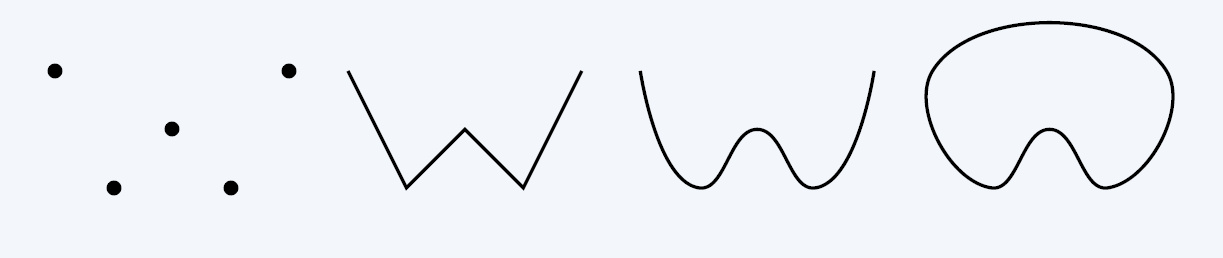
\includegraphics[width=10cm]{images/pstricks4.jpg}

\subsection{Vers les mathématiques}

La combinaison des éléments cités auparavant va permettre d'obtenir des graphiques mathématiques classiques : les flèches formeront les axes, les courbes la plupart des graphiques à tracer, le texte ajoutant des éléments comme les légendes des axes ou le nom des courbes. En général, il convient d'organiser les données numériques à tracer avec des logiciels permettant de concaténer des données en un format accessible à \paquet{pstricks}. En voici un exemple, obtenu avec des coordonnées mises sous forme de $(x_1,y_1)(x_2,y_2)\dots (x_n,y_n)$. 
Le code détaillé de cette figure est placé dans le fichier \macron{3oat.tex} accompagnant le fichier du cours.

\begin{figure}[H]
\centering
\begin{pspicture}(-1,-1)(11,7)
\psline[linewidth=0.01](0,2.286)(0.014,2.293)(0.028,2.34)(0.043,2.347)(0.057,2.349)(0.071,2.337)(0.085,2.322)(0.1,2.318)(0.114,2.327)(0.128,2.322)(0.142,2.297)(0.157,2.289)(0.171,2.306)(0.185,2.292)(0.199,2.206)(0.213,2.182)(0.228,2.159)(0.242,2.158)(0.256,2.157)(0.27,2.166)(0.285,2.154)(0.299,2.137)(0.313,2.124)(0.327,2.147)(0.341,2.143)(0.356,2.141)(0.37,2.136)(0.384,2.115)(0.398,2.127)(0.413,2.13)(0.427,2.122)(0.441,2.134)(0.455,2.144)(0.47,2.141)(0.484,2.139)(0.498,2.16)(0.512,2.148)(0.526,2.147)(0.541,2.139)(0.555,2.15)(0.569,2.159)(0.583,2.157)(0.598,2.144)(0.612,2.159)(0.626,2.159)(0.64,2.142)(0.654,2.146)(0.669,2.119)(0.683,2.123)(0.697,2.12)(0.711,2.117)(0.726,2.122)(0.74,2.136)(0.754,2.133)(0.768,2.13)(0.783,2.128)(0.797,2.144)(0.811,2.143)(0.825,2.135)(0.839,2.149)(0.854,2.163)(0.868,2.153)(0.882,2.144)(0.896,2.145)(0.911,2.14)(0.925,2.114)(0.939,2.119)(0.953,2.139)(0.967,2.126)(0.982,2.106)(0.996,2.102)(1.01,2.101)(1.024,2.099)(1.039,2.111)(1.053,2.073)(1.067,2.084)(1.081,2.083)(1.096,2.097)(1.11,2.08)(1.124,2.088)(1.138,2.117)(1.152,2.156)(1.167,2.15)(1.181,2.15)(1.195,2.147)(1.209,2.119)(1.224,2.103)(1.238,2.068)(1.252,2.076)(1.266,2.081)(1.28,2.08)(1.295,2.072)(1.309,2.051)(1.323,2.057)(1.337,2.005)(1.352,2.004)(1.366,2.001)(1.38,2.033)(1.394,2.042)(1.409,2.017)(1.423,1.982)(1.437,1.945)(1.451,1.919)(1.465,1.946)(1.48,1.919)(1.494,1.935)(1.508,1.912)(1.522,1.901)(1.537,1.879)(1.551,1.845)(1.565,1.899)(1.579,1.902)(1.593,1.904)(1.608,1.887)(1.622,1.914)(1.636,1.938)(1.65,1.927)(1.665,1.923)(1.679,1.926)(1.693,1.888)(1.707,1.839)(1.722,1.834)(1.736,1.803)(1.75,1.762)(1.764,1.746)(1.778,1.727)(1.793,1.705)(1.807,1.712)(1.821,1.727)(1.835,1.749)(1.85,1.696)(1.864,1.656)(1.878,1.599)(1.892,1.615)(1.907,1.588)(1.921,1.592)(1.935,1.65)(1.949,1.629)(1.963,1.604)(1.978,1.628)(1.992,1.641)(2.006,1.644)(2.02,1.613)(2.035,1.637)(2.049,1.699)(2.063,1.699)(2.077,1.691)(2.091,1.665)(2.106,1.667)(2.12,1.678)(2.134,1.726)(2.148,1.78)(2.163,1.798)(2.177,1.87)(2.191,1.906)(2.205,1.906)(2.22,1.895)(2.234,1.897)(2.248,1.943)(2.262,1.898)(2.276,1.925)(2.291,1.899)(2.305,1.878)(2.319,1.85)(2.333,1.868)(2.348,1.828)(2.362,1.844)(2.376,1.866)(2.39,1.899)(2.404,1.91)(2.419,1.861)(2.433,1.825)(2.447,1.795)(2.461,1.753)(2.476,1.755)(2.49,1.787)(2.504,1.78)(2.518,1.793)(2.533,1.779)(2.547,1.765)(2.561,1.8)(2.575,1.805)(2.589,1.818)(2.604,1.792)(2.618,1.817)(2.632,1.806)(2.646,1.786)(2.661,1.802)(2.675,1.768)(2.689,1.752)(2.703,1.735)(2.717,1.708)(2.732,1.691)(2.746,1.686)(2.76,1.667)(2.774,1.634)(2.789,1.623)(2.803,1.622)(2.817,1.606)(2.831,1.559)(2.846,1.551)(2.86,1.53)(2.874,1.525)(2.888,1.529)(2.902,1.529)(2.917,1.529)(2.931,1.45)(2.945,1.45)(2.959,1.447)(2.974,1.45)(2.988,1.504)(3.002,1.515)(3.016,1.507)(3.03,1.493)(3.045,1.46)(3.059,1.435)(3.073,1.411)(3.087,1.413)(3.102,1.392)(3.116,1.369)(3.13,1.369)(3.144,1.307)(3.159,1.28)(3.173,1.282)(3.187,1.285)(3.201,1.27)(3.215,1.223)(3.23,1.236)(3.244,1.263)(3.258,1.24)(3.272,1.249)(3.287,1.226)(3.301,1.226)(3.315,1.135)(3.329,1.082)(3.343,1.088)(3.358,1.083)(3.372,1.074)(3.386,1.071)(3.4,1.016)(3.415,0.979)(3.429,1.021)(3.443,1.038)(3.457,1.06)(3.472,1.016)(3.486,0.995)(3.5,1)(3.514,0.959)(3.528,0.921)(3.543,0.969)(3.557,1.015)(3.571,0.989)(3.585,0.972)(3.6,0.957)(3.614,0.943)(3.628,0.924)(3.642,0.895)(3.657,0.867)(3.671,0.873)(3.685,0.898)(3.699,1.023)(3.713,1.082)(3.728,1.209)(3.742,1.223)(3.756,1.29)(3.77,1.257)(3.785,1.35)(3.799,1.291)(3.813,1.277)(3.827,1.274)(3.841,1.226)(3.856,1.18)(3.87,1.107)(3.884,1.081)(3.898,1.174)(3.913,1.239)(3.927,1.25)(3.941,1.325)(3.955,1.312)(3.97,1.291)(3.984,1.245)(3.998,1.296)(4.012,1.322)(4.026,1.316)(4.041,1.276)(4.055,1.276)(4.069,1.288)(4.083,1.263)(4.098,1.238)(4.112,1.289)(4.126,1.252)(4.14,1.236)(4.154,1.25)(4.169,1.276)(4.183,1.249)(4.197,1.236)(4.211,1.219)(4.226,1.216)(4.24,1.206)(4.254,1.142)(4.268,1.112)(4.283,1.153)(4.297,1.154)(4.311,1.175)(4.325,1.171)(4.339,1.126)(4.354,1.089)(4.368,1.027)(4.382,0.993)(4.396,0.952)(4.411,0.958)(4.425,0.926)(4.439,0.906)(4.453,0.972)(4.467,1.054)(4.482,0.98)(4.496,0.978)(4.51,0.999)(4.524,0.912)(4.539,0.926)(4.553,0.87)(4.567,0.938)(4.581,0.845)(4.596,0.833)(4.61,0.784)(4.624,0.788)(4.638,0.765)(4.652,0.798)(4.667,0.87)(4.681,0.985)(4.695,0.96)(4.709,0.952)(4.724,0.928)(4.738,0.944)(4.752,0.911)(4.766,1.032)(4.78,1.056)(4.795,1.011)(4.809,1.008)(4.823,1.064)(4.837,1.106)(4.852,1.049)(4.866,1.089)(4.88,1.083)(4.894,1.091)(4.909,1.034)(4.923,0.999)(4.937,0.963)(4.951,1.047)(4.965,1.058)(4.98,1.092)(4.994,1.06)(5.008,1.092)(5.022,1.098)(5.037,1.06)(5.051,1.075)(5.065,1.023)(5.079,1.096)(5.093,1.086)(5.108,1.124)(5.122,1.185)(5.136,1.215)(5.15,1.165)(5.165,1.186)(5.179,1.168)(5.193,1.143)(5.207,1.058)(5.222,1.104)(5.236,1.096)(5.25,1.174)(5.264,1.207)(5.278,1.163)(5.293,1.17)(5.307,1.144)(5.321,1.179)(5.335,1.2)(5.35,1.185)(5.364,1.184)(5.378,1.19)(5.392,1.207)(5.407,1.186)(5.421,1.195)(5.435,1.232)(5.449,1.34)(5.463,1.367)(5.478,1.322)(5.492,1.282)(5.506,1.245)(5.52,1.263)(5.535,1.22)(5.549,1.236)(5.563,1.124)(5.577,1.139)(5.591,1.155)(5.606,1.142)(5.62,1.158)(5.634,1.121)(5.648,1.084)(5.663,1.064)(5.677,1.078)(5.691,1.053)(5.705,1.002)(5.72,1.002)(5.734,0.929)(5.748,0.943)(5.762,1.042)(5.776,1.138)(5.791,1.101)(5.805,1.11)(5.819,1.078)(5.833,1.113)(5.848,1.002)(5.862,1.047)(5.876,1.04)(5.89,1.086)(5.904,1.081)(5.919,1.096)(5.933,1.099)(5.947,1.077)(5.961,1.059)(5.976,1.075)(5.99,1.065)(6.004,1.091)(6.018,1.095)(6.033,1.073)(6.047,1.08)(6.061,1.042)(6.075,1.105)(6.089,1.068)(6.104,1.074)(6.118,1.144)(6.132,1.188)(6.146,1.178)(6.161,1.167)(6.175,1.164)(6.189,1.128)(6.203,1.096)(6.217,1.087)(6.232,1.062)(6.246,1.104)(6.26,1.084)(6.274,1.077)(6.289,1.161)(6.303,1.167)(6.317,1.157)(6.331,1.182)(6.346,1.173)(6.36,1.197)(6.374,1.168)(6.388,1.146)(6.402,1.142)(6.417,1.056)(6.431,1.071)(6.445,1.078)(6.459,1.078)(6.474,1.102)(6.488,1.069)(6.502,1.095)(6.516,1.088)(6.53,1.054)(6.545,1.063)(6.559,1.075)(6.573,1.049)(6.587,1.037)(6.602,1.036)(6.616,1.036)(6.63,1.036)(6.644,1.048)(6.659,1.045)(6.673,1.042)(6.687,1.043)(6.701,1.083)(6.715,1.065)(6.73,1.019)(6.744,1.008)(6.758,1.004)(6.772,0.933)(6.787,0.916)(6.801,0.944)(6.815,0.975)(6.829,0.978)(6.843,0.982)(6.858,0.98)(6.872,0.946)(6.886,0.939)(6.9,0.904)(6.915,0.852)(6.929,0.916)(6.943,0.928)(6.957,0.921)(6.972,1.027)(6.986,0.993) \uput[0]{0.1}(7,0.993){La première OAT}
\psline[linewidth=0.02](0,0.27)(0.014,0.288)(0.028,0.344)(0.043,0.362)(0.057,0.374)(0.071,0.372)(0.085,0.368)(0.1,0.374)(0.114,0.393)(0.128,0.398)(0.142,0.383)(0.157,0.385)(0.171,0.412)(0.185,0.408)(0.199,0.332)(0.213,0.318)(0.228,0.306)(0.242,0.315)(0.256,0.324)(0.27,0.343)(0.285,0.341)(0.299,0.334)(0.313,0.331)(0.327,0.365)(0.341,0.371)(0.356,0.379)(0.37,0.384)(0.384,0.373)(0.398,0.395)(0.413,0.408)(0.427,0.41)(0.441,0.432)(0.455,0.453)(0.47,0.46)(0.484,0.468)(0.498,0.499)(0.512,0.497)(0.526,0.506)(0.541,0.508)(0.555,0.53)(0.569,0.549)(0.583,0.557)(0.598,0.554)(0.612,0.579)(0.626,0.589)(0.64,0.582)(0.654,0.597)(0.669,0.579)(0.683,0.594)(0.697,0.601)(0.711,0.608)(0.726,0.623)(0.74,0.647)(0.754,0.654)(0.768,0.661)(0.783,0.669)(0.797,0.696)(0.811,0.705)(0.825,0.707)(0.839,0.731)(0.854,0.756)(0.868,0.756)(0.882,0.757)(0.896,0.768)(0.911,0.773)(0.925,0.757)(0.939,0.772)(0.953,0.802)(0.967,0.799)(0.982,0.789)(0.996,0.795)(1.01,0.804)(1.024,0.812)(1.039,0.835)(1.053,0.807)(1.067,0.828)(1.081,0.838)(1.096,0.861)(1.11,0.855)(1.124,0.873)(1.138,0.912)(1.152,0.961)(1.167,0.965)(1.181,0.975)(1.195,0.982)(1.209,0.964)(1.224,0.958)(1.238,0.934)(1.252,0.952)(1.266,0.967)(1.28,0.976)(1.295,0.978)(1.309,0.967)(1.323,0.983)(1.337,0.942)(1.352,0.951)(1.366,0.958)(1.38,1)(1.394,1.019)(1.409,1.004)(1.423,0.979)(1.437,0.952)(1.451,0.937)(1.465,0.973)(1.48,0.957)(1.494,0.982)(1.508,0.97)(1.522,0.969)(1.537,0.957)(1.551,0.934)(1.565,0.998)(1.579,1.011)(1.593,1.023)(1.608,1.016)(1.622,1.053)(1.636,1.087)(1.65,1.087)(1.665,1.093)(1.679,1.106)(1.693,1.078)(1.707,1.039)(1.722,1.044)(1.736,1.023)(1.75,0.993)(1.764,0.986)(1.778,0.977)(1.793,0.965)(1.807,0.982)(1.821,1.008)(1.835,1.04)(1.85,0.998)(1.864,0.967)(1.878,0.921)(1.892,0.947)(1.907,0.93)(1.921,0.944)(1.935,1.012)(1.949,1.001)(1.963,0.986)(1.978,1.02)(1.992,1.043)(2.006,1.056)(2.02,1.036)(2.035,1.07)(2.049,1.141)(2.063,1.152)(2.077,1.155)(2.091,1.138)(2.106,1.151)(2.12,1.172)(2.134,1.23)(2.148,1.293)(2.163,1.322)(2.177,1.404)(2.191,1.45)(2.205,1.46)(2.22,1.459)(2.234,1.472)(2.248,1.527)(2.262,1.493)(2.276,1.53)(2.291,1.514)(2.305,1.503)(2.319,1.486)(2.333,1.513)(2.348,1.484)(2.362,1.51)(2.376,1.542)(2.39,1.585)(2.404,1.606)(2.419,1.567)(2.433,1.542)(2.447,1.521)(2.461,1.49)(2.476,1.502)(2.49,1.544)(2.504,1.547)(2.518,1.57)(2.533,1.566)(2.547,1.563)(2.561,1.607)(2.575,1.623)(2.589,1.646)(2.604,1.63)(2.618,1.665)(2.632,1.664)(2.646,1.654)(2.661,1.68)(2.675,1.657)(2.689,1.651)(2.703,1.644)(2.717,1.627)(2.732,1.621)(2.746,1.626)(2.76,1.616)(2.774,1.593)(2.789,1.592)(2.803,1.601)(2.817,1.596)(2.831,1.559)(2.846,1.561)(2.86,1.551)(2.874,1.556)(2.888,1.57)(2.902,1.58)(2.917,1.59)(2.931,1.521)(2.945,1.531)(2.959,1.538)(2.974,1.552)(2.988,1.615)(3.002,1.637)(3.016,1.639)(3.03,1.635)(3.045,1.612)(3.059,1.597)(3.073,1.583)(3.087,1.595)(3.102,1.584)(3.116,1.572)(3.13,1.582)(3.144,1.529)(3.159,1.513)(3.173,1.525)(3.187,1.538)(3.201,1.533)(3.215,1.497)(3.23,1.519)(3.244,1.557)(3.258,1.544)(3.272,1.563)(3.287,1.55)(3.301,1.56)(3.315,1.48)(3.329,1.436)(3.343,1.452)(3.358,1.457)(3.372,1.458)(3.386,1.466)(3.4,1.421)(3.415,1.395)(3.429,1.446)(3.443,1.474)(3.457,1.506)(3.472,1.472)(3.486,1.46)(3.5,1.476)(3.514,1.445)(3.528,1.417)(3.543,1.476)(3.557,1.531)(3.571,1.515)(3.585,1.509)(3.6,1.504)(3.614,1.5)(3.628,1.491)(3.642,1.473)(3.657,1.454)(3.671,1.471)(3.685,1.506)(3.699,1.641)(3.713,1.71)(3.728,1.847)(3.742,1.872)(3.756,1.949)(3.77,1.925)(3.785,2.029)(3.799,1.98)(3.813,1.976)(3.827,1.983)(3.841,1.945)(3.856,1.909)(3.87,1.846)(3.884,1.83)(3.898,1.933)(3.913,2.008)(3.927,2.03)(3.941,2.115)(3.955,2.112)(3.97,2.102)(3.984,2.065)(3.998,2.127)(4.012,2.162)(4.026,2.166)(4.041,2.137)(4.055,2.147)(4.069,2.169)(4.083,2.154)(4.098,2.139)(4.112,2.201)(4.126,2.174)(4.14,2.167)(4.154,2.192)(4.169,2.228)(4.183,2.211)(4.197,2.208)(4.211,2.202)(4.226,2.209)(4.24,2.209)(4.254,2.155)(4.268,2.135)(4.283,2.186)(4.297,2.197)(4.311,2.228)(4.325,2.234)(4.339,2.2)(4.354,2.173)(4.368,2.121)(4.382,2.097)(4.396,2.066)(4.411,2.082)(4.425,2.06)(4.439,2.051)(4.453,2.127)(4.467,2.219)(4.482,2.155)(4.496,2.163)(4.51,2.194)(4.524,2.117)(4.539,2.141)(4.553,2.096)(4.567,2.174)(4.581,2.09)(4.596,2.088)(4.61,2.05)(4.624,2.064)(4.638,2.051)(4.652,2.095)(4.667,2.177)(4.681,2.302)(4.695,2.287)(4.709,2.289)(4.724,2.275)(4.738,2.301)(4.752,2.278)(4.766,2.41)(4.78,2.444)(4.795,2.409)(4.809,2.416)(4.823,2.482)(4.837,2.534)(4.852,2.488)(4.866,2.537)(4.88,2.541)(4.894,2.559)(4.909,2.513)(4.923,2.488)(4.937,2.462)(4.951,2.556)(4.965,2.578)(4.98,2.621)(4.994,2.6)(5.008,2.641)(5.022,2.658)(5.037,2.63)(5.051,2.655)(5.065,2.613)(5.079,2.696)(5.093,2.696)(5.108,2.745)(5.122,2.816)(5.136,2.856)(5.15,2.816)(5.165,2.847)(5.179,2.839)(5.193,2.825)(5.207,2.75)(5.222,2.806)(5.236,2.808)(5.25,2.896)(5.264,2.939)(5.278,2.905)(5.293,2.922)(5.307,2.907)(5.321,2.951)(5.335,2.983)(5.35,2.978)(5.364,2.987)(5.378,3.003)(5.392,3.03)(5.407,3.019)(5.421,3.038)(5.435,3.085)(5.449,3.204)(5.463,3.241)(5.478,3.206)(5.492,3.176)(5.506,3.149)(5.52,3.177)(5.535,3.145)(5.549,3.17)(5.563,3.069)(5.577,3.094)(5.591,3.12)(5.606,3.117)(5.62,3.143)(5.634,3.116)(5.648,3.089)(5.663,3.08)(5.677,3.103)(5.691,3.089)(5.705,3.048)(5.72,3.058)(5.734,2.995)(5.748,3.019)(5.762,3.129)(5.776,3.235)(5.791,3.208)(5.805,3.227)(5.819,3.205)(5.833,3.25)(5.848,3.149)(5.862,3.205)(5.876,3.208)(5.89,3.263)(5.904,3.268)(5.919,3.294)(5.933,3.307)(5.947,3.295)(5.961,3.288)(5.976,3.313)(5.99,3.314)(6.004,3.349)(6.018,3.364)(6.033,3.351)(6.047,3.369)(6.061,3.341)(6.075,3.414)(6.089,3.387)(6.104,3.403)(6.118,3.484)(6.132,3.538)(6.146,3.538)(6.161,3.537)(6.175,3.544)(6.189,3.519)(6.203,3.496)(6.217,3.497)(6.232,3.483)(6.246,3.535)(6.26,3.525)(6.274,3.528)(6.289,3.622)(6.303,3.638)(6.317,3.638)(6.331,3.674)(6.346,3.675)(6.36,3.709)(6.374,3.69)(6.388,3.678)(6.402,3.685)(6.417,3.609)(6.431,3.633)(6.445,3.65)(6.459,3.66)(6.474,3.695)(6.488,3.672)(6.502,3.708)(6.516,3.711)(6.53,3.688)(6.545,3.707)(6.559,3.728)(6.573,3.713)(6.587,3.711)(6.602,3.72)(6.616,3.73)(6.63,3.74)(6.644,3.763)(6.659,3.77)(6.673,3.777)(6.687,3.788)(6.701,3.838)(6.715,3.831)(6.73,3.794)(6.744,3.793)(6.758,3.799)(6.772,3.738)(6.787,3.731)(6.801,3.77)(6.815,3.811)(6.829,3.824)(6.843,3.839)(6.858,3.847)(6.872,3.822)(6.886,3.825)(6.9,3.801)(6.915,3.759)(6.929,3.833)(6.943,3.855)(6.957,3.858)(6.972,3.974)(6.986,3.95) \uput[0]{0.1}(7,3.95){La deuxième OAT}
\psline[linewidth=0.03](0,0.591)(0.014,0.64)(0.028,0.654)(0.043,0.735)(0.057,0.769)(0.071,0.852)(0.085,0.921)(0.1,0.99)(0.114,1.058)(0.128,1.154)(0.142,1.207)(0.157,1.235)(0.171,1.309)(0.185,1.34)(0.199,1.391)(0.213,1.407)(0.228,1.436)(0.242,1.511)(0.256,1.55)(0.27,1.576)(0.285,1.666)(0.299,1.725)(0.313,1.783)(0.327,1.792)(0.341,1.812)(0.356,1.829)(0.37,1.878)(0.384,1.883)(0.398,1.947)(0.413,2.003)(0.427,2.024)(0.441,2.106)(0.455,2.175)(0.47,2.19)(0.484,2.288)(0.498,2.308)(0.512,2.317)(0.526,2.405)(0.541,2.477)(0.555,2.524)(0.569,2.575)(0.583,2.583)(0.598,2.58)(0.612,2.605)(0.626,2.615)(0.64,2.608)(0.654,2.622)(0.669,2.605)(0.683,2.619)(0.697,2.626)(0.711,2.633)(0.726,2.649)(0.74,2.673)(0.754,2.68)(0.768,2.687)(0.783,2.695)(0.797,2.721)(0.811,2.731)(0.825,2.733)(0.839,2.757)(0.854,2.781)(0.868,2.781)(0.882,2.782)(0.896,2.793)(0.911,2.798)(0.925,2.782)(0.939,2.797)(0.953,2.828)(0.967,2.825)(0.982,2.815)(0.996,2.821)(1.01,2.83)(1.024,2.838)(1.039,2.86)(1.053,2.833)(1.067,2.854)(1.081,2.863)(1.096,2.887)(1.11,2.88)(1.124,2.899)(1.138,2.937)(1.152,2.987)(1.167,2.991)(1.181,3.001)(1.195,3.008)(1.209,2.99)(1.224,2.984)(1.238,2.959)(1.252,2.978)(1.266,2.993)(1.28,3.002)(1.295,3.004)(1.309,2.993)(1.323,3.009)(1.337,2.968)(1.352,2.977)(1.366,2.984)(1.38,3.025)(1.394,3.045)(1.409,3.029)(1.423,3.005)(1.437,2.978)(1.451,2.963)(1.465,2.999)(1.48,2.983)(1.494,3.008)(1.508,2.996)(1.522,2.995)(1.537,2.983)(1.551,2.959)(1.565,3.023)(1.579,3.036)(1.593,3.049)(1.608,3.042)(1.622,3.079)(1.636,3.112)(1.65,3.112)(1.665,3.119)(1.679,3.132)(1.693,3.103)(1.707,3.065)(1.722,3.07)(1.736,3.049)(1.75,3.018)(1.764,3.012)(1.778,3.003)(1.793,2.991)(1.807,3.008)(1.821,3.033)(1.835,3.066)(1.85,3.023)(1.864,2.993)(1.878,2.946)(1.892,2.973)(1.907,2.955)(1.921,2.97)(1.935,3.037)(1.949,3.026)(1.963,3.012)(1.978,3.046)(1.992,3.069)(2.006,3.082)(2.02,3.062)(2.035,3.095)(2.049,3.167)(2.063,3.177)(2.077,3.18)(2.091,3.164)(2.106,3.176)(2.12,3.198)(2.134,3.255)(2.148,3.319)(2.163,3.347)(2.177,3.429)(2.191,3.476)(2.205,3.486)(2.22,3.485)(2.234,3.497)(2.248,3.553)(2.262,3.519)(2.276,3.556)(2.291,3.54)(2.305,3.529)(2.319,3.511)(2.333,3.539)(2.348,3.509)(2.362,3.536)(2.376,3.567)(2.39,3.611)(2.404,3.632)(2.419,3.593)(2.433,3.567)(2.447,3.547)(2.461,3.516)(2.476,3.528)(2.49,3.569)(2.504,3.572)(2.518,3.596)(2.533,3.591)(2.547,3.588)(2.561,3.633)(2.575,3.648)(2.589,3.672)(2.604,3.655)(2.618,3.691)(2.632,3.69)(2.646,3.68)(2.661,3.706)(2.675,3.683)(2.689,3.677)(2.703,3.669)(2.717,3.652)(2.732,3.646)(2.746,3.651)(2.76,3.642)(2.774,3.619)(2.789,3.618)(2.803,3.627)(2.817,3.622)(2.831,3.584)(2.846,3.586)(2.86,3.576)(2.874,3.581)(2.888,3.596)(2.902,3.606)(2.917,3.616)(2.931,3.547)(2.945,3.557)(2.959,3.564)(2.974,3.577)(2.988,3.641)(3.002,3.662)(3.016,3.664)(3.03,3.66)(3.045,3.638)(3.059,3.623)(3.073,3.609)(3.087,3.621)(3.102,3.61)(3.116,3.598)(3.13,3.608)(3.144,3.555)(3.159,3.539)(3.173,3.551)(3.187,3.564)(3.201,3.559)(3.215,3.523)(3.23,3.545)(3.244,3.582)(3.258,3.569)(3.272,3.588)(3.287,3.575)(3.301,3.585)(3.315,3.505)(3.329,3.462)(3.343,3.478)(3.358,3.483)(3.372,3.484)(3.386,3.491)(3.4,3.447)(3.415,3.42)(3.429,3.472)(3.443,3.499)(3.457,3.532)(3.472,3.497)(3.486,3.486)(3.5,3.501)(3.514,3.471)(3.528,3.443)(3.543,3.501)(3.557,3.557)(3.571,3.541)(3.585,3.535)(3.6,3.53)(3.614,3.526)(3.628,3.517)(3.642,3.498)(3.657,3.48)(3.671,3.496)(3.685,3.532)(3.699,3.666)(3.713,3.735)(3.728,3.873)(3.742,3.897)(3.756,3.974)(3.77,3.951)(3.785,4.054)(3.799,4.006)(3.813,4.002)(3.827,4.009)(3.841,3.97)(3.856,3.935)(3.87,3.872)(3.884,3.856)(3.898,3.959)(3.913,4.034)(3.927,4.055)(3.941,4.14)(3.955,4.137)(3.97,4.127)(3.984,4.091)(3.998,4.153)(4.012,4.188)(4.026,4.192)(4.041,4.163)(4.055,4.173)(4.069,4.195)(4.083,4.18)(4.098,4.165)(4.112,4.227)(4.126,4.199)(4.14,4.193)(4.154,4.217)(4.169,4.254)(4.183,4.237)(4.197,4.234)(4.211,4.228)(4.226,4.235)(4.24,4.235)(4.254,4.181)(4.268,4.161)(4.283,4.211)(4.297,4.222)(4.311,4.254)(4.325,4.26)(4.339,4.226)(4.354,4.198)(4.368,4.147)(4.382,4.122)(4.396,4.092)(4.411,4.108)(4.425,4.086)(4.439,4.077)(4.453,4.153)(4.467,4.245)(4.482,4.181)(4.496,4.189)(4.51,4.219)(4.524,4.142)(4.539,4.167)(4.553,4.121)(4.567,4.199)(4.581,4.116)(4.596,4.114)(4.61,4.076)(4.624,4.09)(4.638,4.077)(4.652,4.12)(4.667,4.202)(4.681,4.328)(4.695,4.313)(4.709,4.315)(4.724,4.3)(4.738,4.327)(4.752,4.304)(4.766,4.435)(4.78,4.47)(4.795,4.434)(4.809,4.441)(4.823,4.508)(4.837,4.56)(4.852,4.513)(4.866,4.563)(4.88,4.567)(4.894,4.585)(4.909,4.538)(4.923,4.513)(4.937,4.488)(4.951,4.582)(4.965,4.603)(4.98,4.647)(4.994,4.626)(5.008,4.667)(5.022,4.683)(5.037,4.656)(5.051,4.68)(5.065,4.639)(5.079,4.722)(5.093,4.722)(5.108,4.77)(5.122,4.841)(5.136,4.882)(5.15,4.841)(5.165,4.873)(5.179,4.865)(5.193,4.85)(5.207,4.775)(5.222,4.831)(5.236,4.833)(5.25,4.921)(5.264,4.965)(5.278,4.93)(5.293,4.948)(5.307,4.932)(5.321,4.977)(5.335,5.008)(5.35,5.003)(5.364,5.012)(5.378,5.029)(5.392,5.056)(5.407,5.045)(5.421,5.064)(5.435,5.111)(5.449,5.229)(5.463,5.267)(5.478,5.231)(5.492,5.202)(5.506,5.175)(5.52,5.203)(5.535,5.17)(5.549,5.196)(5.563,5.095)(5.577,5.12)(5.591,5.145)(5.606,5.143)(5.62,5.168)(5.634,5.142)(5.648,5.115)(5.663,5.106)(5.677,5.129)(5.691,5.115)(5.705,5.073)(5.72,5.083)(5.734,5.021)(5.748,5.045)(5.762,5.154)(5.776,5.261)(5.791,5.233)(5.805,5.253)(5.819,5.23)(5.833,5.276)(5.848,5.175)(5.862,5.23)(5.876,5.233)(5.89,5.289)(5.904,5.294)(5.919,5.319)(5.933,5.333)(5.947,5.32)(5.961,5.313)(5.976,5.339)(5.99,5.34)(6.004,5.375)(6.018,5.389)(6.033,5.377)(6.047,5.394)(6.061,5.367)(6.075,5.44)(6.089,5.413)(6.104,5.429)(6.118,5.51)(6.132,5.563)(6.146,5.563)(6.161,5.562)(6.175,5.57)(6.189,5.544)(6.203,5.522)(6.217,5.523)(6.232,5.509)(6.246,5.56)(6.26,5.55)(6.274,5.553)(6.289,5.648)(6.303,5.664)(6.317,5.664)(6.331,5.699)(6.346,5.7)(6.36,5.735)(6.374,5.715)(6.388,5.703)(6.402,5.71)(6.417,5.634)(6.431,5.659)(6.445,5.676)(6.459,5.686)(6.474,5.72)(6.488,5.697)(6.502,5.734)(6.516,5.737)(6.53,5.713)(6.545,5.733)(6.559,5.754)(6.573,5.739)(6.587,5.737)(6.602,5.746)(6.616,5.756)(6.63,5.766)(6.644,5.788)(6.659,5.795)(6.673,5.802)(6.687,5.814)(6.701,5.863)(6.715,5.856)(6.73,5.82)(6.744,5.819)(6.758,5.825)(6.772,5.764)(6.787,5.757)(6.801,5.795)(6.815,5.837)(6.829,5.85)(6.843,5.864)(6.858,5.872)(6.872,5.848)(6.886,5.851)(6.9,5.827)(6.915,5.784)(6.929,5.858)(6.943,5.88)(6.957,5.884)(6.972,6)(6.986,5.976) \uput[0]{0.1}(7,5.976){La dernière OAT}
\psline{->}(-0.1,0)(7.2,0)
\uput[0](7.4,0){Date}
\psline{->}(0,-0.1)(0,6.2)
\rput(0,6.5){Taux}
\psline(-0.1,1.013)(0.1,1.013) \uput[180]{0}(-0.1,1.013){2\%}\psline(-0.1,2.026)(0.1,2.026) \uput[180]{0}(-0.1,2.026){3\%}\psline(-0.1,3.038)(0.1,3.038) \uput[180]{0}(-0.1,3.038){4\%}\psline(-0.1,4.051)(0.1,4.051) \uput[180]{0}(-0.1,4.051){5\%}\psline(-0.1,5.064)(0.1,5.064) \uput[180]{0}(-0.1,5.064){6\%}

\psline(0,-0.1)(0,0.1) \uput[270]{45}(0,-0.1){3/99}\psline(0.868,-0.1)(0.868,0.1) \uput[270]{45}(0.868,-0.1){5/99}\psline(1.736,-0.1)(1.736,0.1) \uput[270]{45}(1.736,-0.1){7/99}\psline(2.618,-0.1)(2.618,0.1) \uput[270]{45}(2.618,-0.1){9/99}\psline(3.486,-0.1)(3.486,0.1) \uput[270]{45}(3.486,-0.1){11/99}\psline(4.354,-0.1)(4.354,0.1) \uput[270]{45}(4.354,-0.1){1/00}\psline(5.207,-0.1)(5.207,0.1) \uput[270]{45}(5.207,-0.1){3/00}\psline(6.075,-0.1)(6.075,0.1) \uput[270]{45}(6.075,-0.1){5/00}\psline(6.986,-0.1)(6.986,0.1) \uput[270]{45}(6.986,-0.1){7/00}

\end{pspicture}
\caption{Quelques OAT}\label{3oat}
\end{figure}

%%%% Ajout YT récent %%%% 
\subsection{Le tracé de fonction mathématique}

Le paquet \paquet{pst-plot}, un des paquets spécialisés se basant sur \paquet{pstricks}, contient quelques  commandes de traçage non négligeables. La plus simple,\macro{psaxes}, trace des axes à nos figures.

\subsubsection{La notation des fonctions}

L'appel du paquet \paquet{pst-plot} permet d'utiliser en particulier les notations mathématiques usuelles avec l'option \macron{algebraic=true} à placer parmi les options des commandes \macro{psplot} et \macro{parametricplot}, comme l'illustrent les exemples qui suivent. Sans cette option, les notations doivent se faire selon une notation polonaise inversée\footnote{Cette notation n'utilise pas la notion de parenthèses. Pour cela, les opérateurs se placent après les opérandes sur lesquels ils s'appliquent. Plus exactement, les termes se lisent successivement : si un terme est un opérande, il est stocké. Si c'est un opérateur, il s'applique aux derniers opérandes stockés.}.

La notation\footnote{Voir par exemple \liensimple{http://ww2.ac-poitiers.fr/math/spip.php?article134&debut_page=1}.} travaille en radian et non en degré. Dans le cas d'une  commande paramétrique, la variable muette est \macron{t} et il faut indiquer une séparation avec un \macron{|} entre les deux fonctions paramétriques du \macro{parametricplot}.

\subsubsection{Une fonction classique}

Voici donc l'exemple de la fonction $sin (2x)$.

\codefigure{
\macro{begin}\{pspicture\}(-1,-1.25)(7,1.25) \\
\macro{psplot}[plotstyle=curve,plotpoints=199,linecolor=bleu8,algebraic=true]\{0\}\{6\}\{sin(2*x)\} \\
\macro{psaxes}(0,0)(-0.5,-1.25)(6.25,1.25) \\
\macro{end}\{pspicture\}
}{
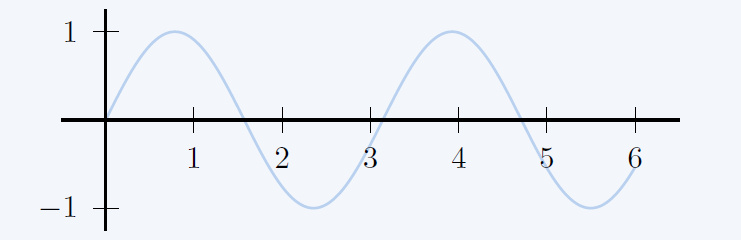
\includegraphics[width=8cm]{images/sinus.jpg}
%\begin{pspicture}(-1,-1.25)(7,1.25)
%\psplot[plotstyle=curve,plotpoints=199,linecolor=bleu8,algebraic=true]{0}{6}{sin(2*x)}
%\psaxes(0,0)(-0.5,-1.25)(6.5,1.25)
%\end{pspicture}
}{Une sinusoïde}

L'option \macron{plotpoints} indique de plus le nombre de points à calculer pour tracer la courbe. Par ailleurs, l'option \macron{plotstyle} permet de préciser avec la valeur \macron{curve} que le tracé de la fonction se fait par courbe, autrement dit qu'il est lissé (il pourrait se faire par ligne avec la valeur \macron{line} ou par de simples points avec \macron{dots}). 

\subsubsection{Une fonction paramétrique}

Pour des fonctions paramétrées, il faut mettre à la suite les fonctions de chaque coordonnées l'une après l'autre, \LaTeX\ repérant les deux fonctions du fait de la notation polonaise inversée. Voici l'exemple d'une rosace avec \macro{parametricplot} :

$$
\left\{
\begin{array}{lcr}
x(t)&=& 2 \sin 4t \cos 5t \\
y(t)&=& 2 \cos 4t \cos 5t 
\end{array}
\right.
$$

\codefigure{
\macro{begin}\{pspicture\}(-2.15,-2.15)(2.15,2.15)  \\
\macro{parametricplot}[plotstyle=curve,plotpoints=199,linecolor=bleu8,algebraic=true]\{0\}\{6.3\}\\\{2*(sin(4*t))*(cos(5*t))|2*(cos(4*t))*(cos(5*t))\} \\
\macro{psaxes}(0,0)(-2.1,-2.1)(2.1,2.1) \\
\macro{end}\{pspicture\}
}{
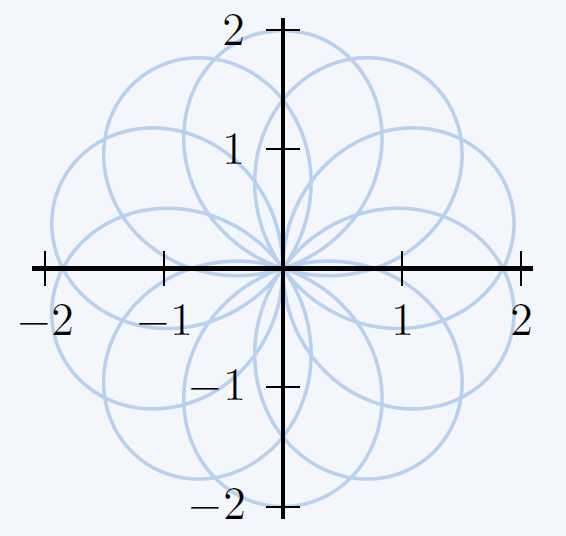
\includegraphics[width=4.3cm]{images/rosace.jpg}
%\begin{pspicture}(-2.15,-2.15)(2.15,2.15)
%\parametricplot[plotstyle=curve,plotpoints=199,linecolor=bleu8,algebraic=true]{0}{6.3}{2*(sin(4*t))*(cos(5*t))|2*(cos(4*t))*(cos(5*t))}
%\psaxes(0,0)(-2.1,-2.1)(2.1,2.1)
%\end{pspicture}
}{Une rosace}


\subsection{Exemples capillotractés} 

\subsubsection{Un histogramme}

Les  commandes de \paquet{pstricks} peuvent être combinées encore plus fortement, jusqu'à définir un ensemble de  commandes dédiées à des traitements particuliers. Il faut ici combiner utilisation de \paquet{pstricks} et programmation.

Voici, pour illustrer ce point, un histogramme obtenu avec un paquet inconnu car fait maison : \paquet{histogra}\footnote{Ce paquet est très peu documenté et encore moins développé pour servir partout... il n'a servi que pour réaliser quelques figures dans un document bien précis.}.

%\sethisto{inter=0,large=0.25,hcol1=bleu5}

\begin{figure}[H]
\begin{center}
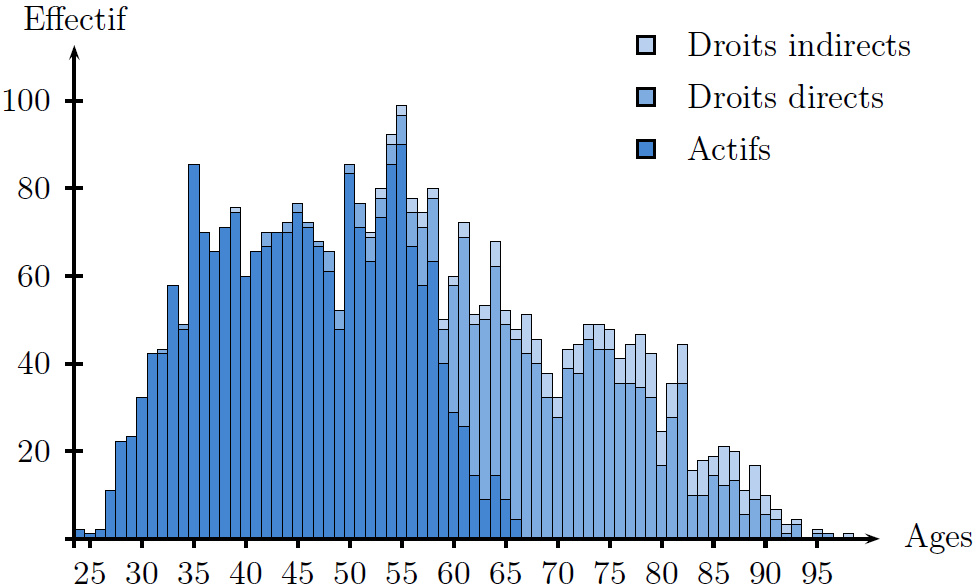
\includegraphics[width=11cm]{images/histogra.jpg}
%\begin{pspicture}(-0.5,-0.5)(10.5,6.5)
%
%\psset{dimen=middle,fillstyle=solid}
%\psframe[fillcolor=bleu8](6.5,5.6)(6.7,5.8) \uput[0]{0}(6.9,5.7){Droits indirects}
%\psframe[fillcolor=bleu7](6.5,5)(6.7,5.2)   \uput[0]{0}(6.9,5.1){Droits directs}
%\psframe[fillcolor=bleu6](6.5,4.4)(6.7,4.6) \uput[0]{0}(6.9,4.5){Actifs}
%
%\essai[inter=0,large=0.12,hcol1=bleu6,hcol2=bleu7,hcol3=bleu8,epais=0.3pt]{(0.2,0,0)(0.1,0,0)(0.2,0,0)(1,0,0)(2,0,0)(2.1,0,0)(2.9,0,0)(3.8,0,0)(3.8,0.1,0)(5.2,0,0)(4.3,0.1,0)(7.7,0,0)(6.3,0,0)(5.9,0,0)(6.4,0,0)(6.7,0,0.1)(5.4,0,0)(5.9,0,0)(6,0.3,0)(6.3,0,0)(6.3,0.2,0)(6.7,0.2,0)(6.4,0.1,0)(6,0.1,0)(5.5,0.4,0)(4.3,0.4,0)(7.5,0.2,0)(6.4,0.5,0)(5.7,0.5,0.1)(6.6,0.4,0.2)(7.7,0.4,0.2)(8.1,0.6,0.2)(6,0.7,0.3)(5.2,1.2,0.3)(5.7,1.3,0.2)(3.6,0.7,0.2)(2.6,2.6,0.2)(2.3,3.9,0.3)(1.3,3.1,0.2)(0.8,3.7,0.3)(1.3,4.3,0.5)(0.8,3.6,0.3)(0.4,3.7,0.2)(0,3.8,0.8)(0,3.6,0.5)(0,2.9,0.5)(0,2.5,0.4)(0,3.5,0.4)(0,3.4,0.6)(0,4.1,0.3)(0,3.9,0.5)(0,3.9,0.4)(0,3.2,0.5)(0,3.2,0.8)(0,3.1,1.1)(0,2.9,0.9)(0,1.5,0.7)(0,2.5,0.7)(0,3.2,0.8)(0,0.9,0.5)(0,0.9,0.7)(0,1.3,0.4)(0,1.1,0.8)(0,1.2,0.6)(0,0.5,0.5)(0,0.8,0.7)(0,0.5,0.4)(0,0.4,0.2)(0,0.1,0.2)(0,0.3,0.1)(0,0,0)(0,0.1,0.1)(0,0.1,0)(0,0,0)(0,0,0.1)(0,0,0)}
%
%\psset{linewidth=1pt}
%\axex(9.3,Ages)
%\axey(5.7,Effectif)
%
%\end{pspicture}
\end{center}
\caption{Pyramide des effectifs}
\end{figure}

%\end{document}

\subsubsection{Une famille de courbes} \label{famillecourbe}

Ce qui suit utilise un mélange de commandes tirées des paquets \paquet{pstricks} et \paquet{multido}. Est tracé ici une famille de figures paramétrées définie par le système suivant :

$$
\left\{
\begin{array}{lcr}
x(t)&=& 0,9 \cos \alpha t \\
y(t)&=& 0,9 \sin \beta t  
\end{array}  \quad \textrm{avec } (\alpha,\beta) \in [1..5]\times[1..6]
\right.
$$

Pour faire ce tracé, une commande un peu plus générale est définie. Dans celle-ci, \paquet{multido} permet de faire deux boucles imbriquées (une sur $\alpha$, l'autre sur $\beta$) et \paquet{pst-plot} permet de tracer la figure voulue.

\begin{codesimple}{Construction d'une famille de courbes}{codfamillecourbe}
\newcommand{\figu}[1]{
\begin{figure}[H]
\begin{center}
\fbox{
\begin{pspicture}(12.3,15.2)
  \multido{\Na=1.1+2.5,\Ia=1+1}{5}{
    \multido{\Nb=13.9+-2.5,\Ib=1+1}{6}{
      \rput{0}(\Na,\Nb){
        \parametricplot[plotstyle=curve,plotpoints=199,linecolor=bleu6,
        algebraic=true]{0}{6.2832}{#1}
        \rput{0}(0,-1.2){\textsf{\footnotesize (\Ia,\Ib)}}}
}}
\end{pspicture}}
\caption{Exemples de fonctions paramétriques}
\end{center}
\end{figure}}
\end{codesimple}


Ainsi, l'utilisation de la  commande s'est limitée à l'appel qui suit. Cependant, en terme de présentation, cette  commande devrait disposer de plus de paramètres que les formules. Sans cela, la légende, le nombre de figures tracées et leur précision ne peuvent être modifiés aisément.

\begin{codesimple}{Appel de la  commande pour les courbes}{appelcourbes}
\figu{0.9*cos(t*\Ia)|0.9*sin(t*\Ib)}
\end{codesimple}


% Ci-dessous la fonction générale
\newcommand{\figu}[1]{
\begin{figure}[H]
\begin{center}
\fbox{
\begin{pspicture}(12.3,15.2)
  \multido{\Na=1.1+2.5,\Ia=1+1}{5}{
    \multido{\Nb=13.9+-2.5,\Ib=1+1}{6}{
      \rput{0}(\Na,\Nb){
        \parametricplot[plotstyle=curve,plotpoints=199,linecolor=bleu6,algebraic=true]{0}{6.2832}{#1}
        \rput{0}(0,-1.2){\textsf{\footnotesize (\Ia,\Ib)}}}
}}
\end{pspicture}}
$$
\left\{
\begin{array}{lcr}
x(t)&=& 0,9 \cos \alpha t \\
y(t)&=& 0,9 \sin \beta t  
\end{array}  \quad \textrm{avec } (\alpha,\beta) \in [1..5]\times[1..6]
\right.
$$
\caption{Exemples de fonctions paramétriques}
\end{center}
\end{figure}
}

%\figu{0.9*cos(t*\Ia)|0.9*sin(t*\Ib)} 

\begin{figure}[H]
\begin{center}
\fbox{%
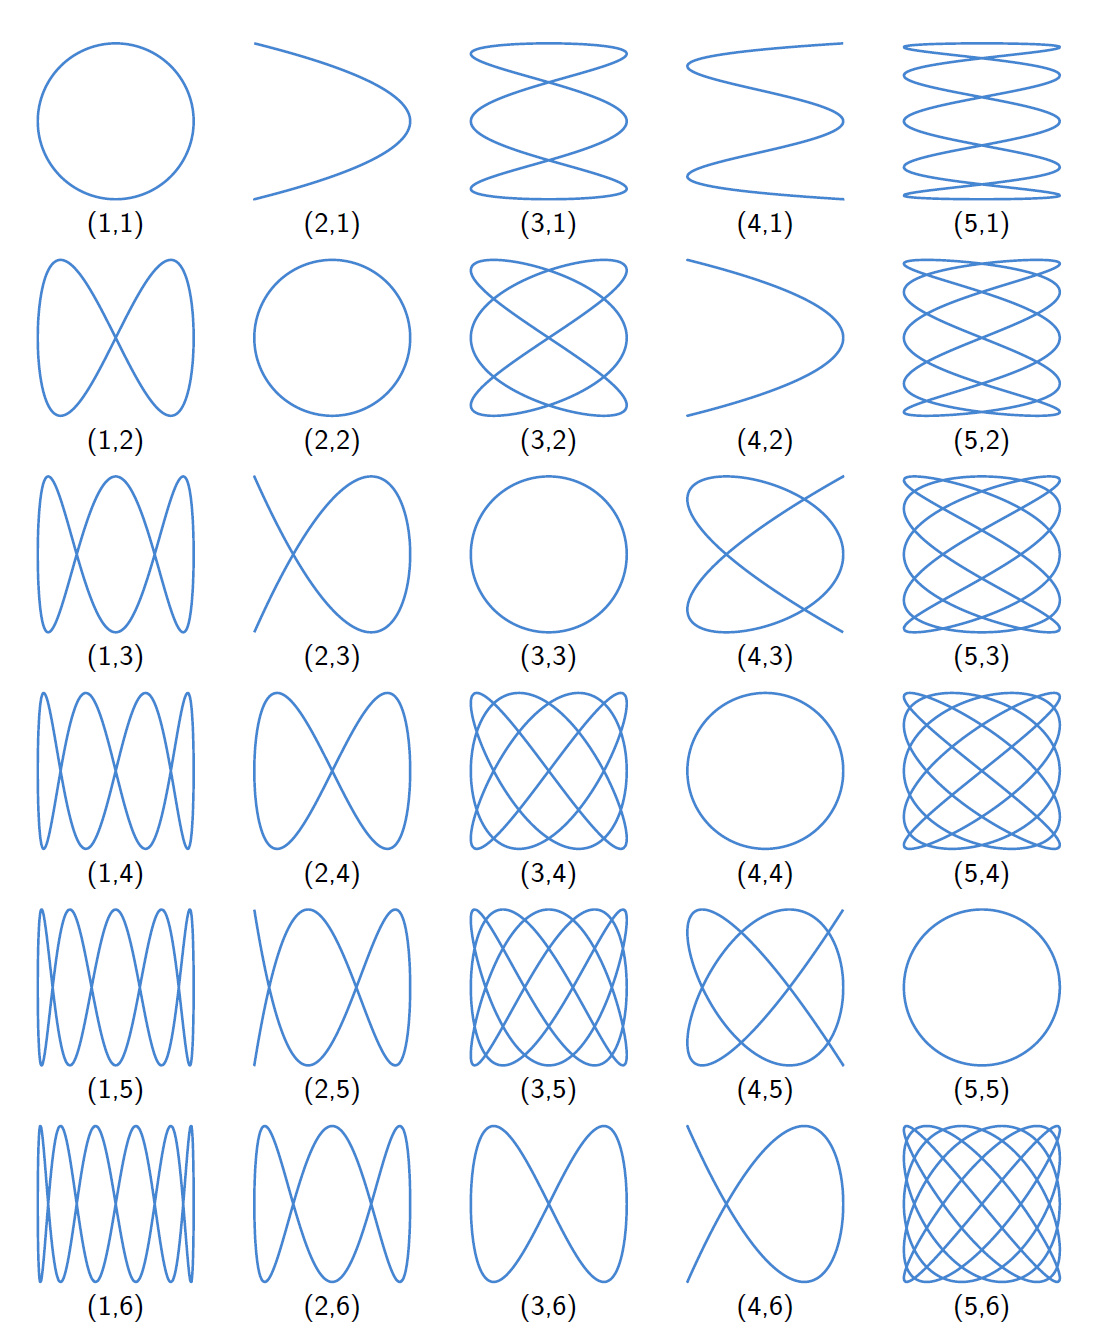
\includegraphics[width=11cm]{images/planche.jpg}%
}
\caption{Exemples de fonctions paramétriques}
\end{center}
\end{figure}


\section{Tikz} \label{tikz} %\incise{---}{---}{---}

Le paquet \paquet{tikz} est plus récent que le paquet \paquet{pstricks}. Par rapport à ce dernier, il présente deux avantages :
\begin{itemize}
\item il dispose généralement de plus grandes possibilités de paramétrages ;
\item il fonctionne avec les différentes chaînes générant directement des fichiers \dextension{pdf}, ce qui en fait la solution graphique pour les fichiers image \dextension{jpg} mais aussi avec les variantes de \LaTeX{} que sont \XeLaTeX{} et Lua\LaTeX.
\end{itemize}

En contrepartie, il demande un peu plus de temps pour être utilisé. Par ailleurs, sur des graphiques nécessitant des calculs, il est plus lent que \paquet{pstricks}, ce dernier bénéficiant des mécaniques propres au langage postscript.

Ce paquet met à disposition un environnement pour traiter les figures : 
\begin{codesimple}{L'environnement de \pseudopaquet{tikz}}{environnementtikz}
\begin{tikzpicture}[§oc£¤options§fc] 
% Figure tikz
\end{tikzpicture}
\end{codesimple}


Cet environnement ne nécessite pas, contrairement à celui de \paquet{pstricks} de dimension : \paquet{tikz} va déterminer les dimensions de la zone à afficher pour qu'elle contienne et affiche l'ensemble des objets tracés\footnote{Ce comportement peut se piloter. Il suffit de placer des n\oe{}uds délimitant une zone plus large pour forcer \paquet{tikz} à suivre d'éventuels besoins de présentation.}. Qui plus est, \paquet{tikz} prend en compte d'éventuelles\textit{options} : ces dernières vont s'appliquer à l'ensemble des objets décrits par la suite, sauf règle explicite contraire présente dans un objet ou une classe d'objets.

\subsection{Le placement par les n\oe{}uds}

Sous \paquet{tikz}, les éléments sont placés sur un n\oe ud (\emph{node}). Un n\oe ud peut être défini par des coordonnées ou de façon relative à d'autres points. Il peut également être appelé par son nom.

\codefigure{
\macro{begin}\{tikzpicture\}[outer sep=0cm,inner sep=0cm] \\
\macro{node} (aa) at (1,0.5) \{1.\macro{LaTeX}\}; \\
\macro{node} (ab) at (0.8,1.1) \{\}; \\
\macro{node}[anchor=south west] at (ab) \{\macro{resizebox}\{3.5cm\}\{!\}\{2.\macro{textcolor}\{bleu5\}\{\macro{LaTeX}\}\}\}; \\
\macro{node}[rotate=160] (ac) at (8,1.1) \{\macro{resizebox}\{!\}\{0.7cm\}\{3.\macro{LaTeX}\}\}; \\
\macro{node} (ad) at (6,1) \{\}; \\
\macro{node}[anchor=north east,outer sep=0cm,inner sep=0cm] at (ad) \{\macro{resizebox}\{!\}\{0.6cm\}\{\macro{reflectbox}\{4.\macro{LaTeX}\}\}\}; \\
%\draw[color=bleu6] plot[only marks,mark=x] coordinates{(aa)(ab)(ac)(ad)};
\macro{end}\{tikzpicture\}
}{
\fontfamily{lmr}\selectfont
\begin{tikzpicture}[outer sep=0cm,inner sep=0cm]
\node (a) at (0,0) {}; \node (b) at (10,2) {}; % pour dimensionner l'image
\node (aa) at (1,0.5) {1.\LaTeX};
\node (ab) at (0.8,1.1) {};
\node[anchor=south west] at (ab) {\resizebox{3.5cm}{!}{2.\textcolor{bleu5}{\LaTeX}}};
\node[rotate=160] (ac) at (8,1.1) {\resizebox{!}{0.7cm}{3.\LaTeX}};
\node (ad) at (6,1) {};
\node[anchor=north east,outer sep=0cm,inner sep=0cm] at (ad) {\resizebox{!}{0.6cm}{\reflectbox{4.\LaTeX}}};
\draw[color=bleu6] plot[only marks,mark=x] coordinates{(aa)(ab)(ac)(ad)};
\end{tikzpicture}
}{Placements et redimensionnements}

\subsection{Les boîtes ou formes}

Différentes formes sont prédéfinies sous \paquet{tikz}\footnote{en particulier avec la bibliothèque \emph{shape} qui définit par exemple le losange utilisé dans l'exemple.}. Se retrouve ici la logique de préciser le tracé du pourtour, le remplissage de la forme, la présence d'une ombre, que ce soit pour la couleur, l'épaisseur, les motifs...). 

De nombreuses valeurs sont disponibles sous forme de mots clés. Par exemple, \macron{thick} utilisé dans l'exemple définit un trait de 0,8pt d'épaisseur.

\codefigure{
\macro{begin}\{tikzpicture\} \\
\macro{node}[rectangle,draw] at (2,1) \{1.\macro{LaTeX}\}; \\
\macro{node}[rectangle,fill=bleu6,drop shadow] at (5,0.5) \{2.\macro{LaTeX}\}; \\
\macro{node}[diamond,aspect=2.5,draw=bleu6,thick] at (5,1.5) \{3.\macro{LaTeX}\}; \\
\macro{node}[circle,draw=bleu6,loosely dotted,thick] at (8,1) \{\macro{Large} 4.\macro{LaTeX}\}; \\
\macro{end}\{tikzpicture\}
}{
\fontfamily{lmr}\selectfont
\begin{tikzpicture}%[outer sep=0cm,inner sep=0cm]
\node (a) at (0,0) {}; \node (b) at (10,2) {}; 
\node[rectangle,draw] at (2,1) {1.\LaTeX}; 
\node[rectangle,fill=bleu6,drop shadow] at (5,0.5) {2.\LaTeX}; 
\node[diamond,aspect=2.5,draw=bleu6,thick] at (5,1.5) {3.\LaTeX}; 
\node[circle,draw=bleu6,loosely dotted,thick] at (8,1) {\Large 4.\LaTeX}; 
\end{tikzpicture}
}{Boîtes}

\subsection{Les grilles}

Les grilles se présentent sous une forme un peu différente de celle vue dans \paquet{pstricks}. En effet, la fonctionnalité la plus courante ne propose pas la numérotation des axes ; de même la grille se base sur les coordonnées du plan ce qui fait que la seconde grille ci-dessous ne commence pas par un filet vertical. 

\begin{codedoublefig}{Grilles}{tikzgrilles}
\begin{tikzpicture}%[outer sep=0cm,inner sep=0cm]
\node (a) at (0,0) {}; \node (b) at (10,2) {}; 
\draw[step=.2cm,gray,very thin] (0,0) grid (2,1.4);
\draw[step=1cm] (0,0) grid (2,1.4);
\draw (3.5,0) grid[xstep=0.4cm,ystep=0.5cm] (5.5,1.4);
\end{tikzpicture}
\end{codedoublefig}

Par contre, lorsqu'il s'agit de traiter la représentation de données, \paquet{tikz} dispose de commandes avancées pour traiter ce point.

\subsection{Les points et courbes}

De la même manière, \paquet{pstricks} dispose de plusieurs commandes de base pour former des traits anguleux, curvilignes. L'exemple suivant les présente sans option.

\begin{codedoublefig}{Points et courbes}{tikzpoints}
\begin{tikzpicture}%[outer sep=0cm,inner sep=0cm]
\node (a) at (0,0) {}; \node (b) at (10,2) {}; 
\fill (0,1) circle (2pt);
\fill (0.5,0) circle (2pt);
\fill (1,0.5) circle (2pt);
\fill (1.5,0) circle (2pt);
\fill (2,1) circle (2pt);
\draw (2.5,1) -- (3,0) -- (3.5,0.5) -- (4,0) -- (4.5,1);
\draw plot[smooth] coordinates{(5,1) (5.5,0) (6,0.5) (6.5,0) (7,1)};
\draw plot[smooth cycle,tension=0.8] coordinates{(7.5,1) (8,0) (8.5,0.5) (9,0) (9.5,1)};
\end{tikzpicture}
\end{codedoublefig}


\alerte{Présentation à poursuivre}

